\documentclass[a4paper]{article}
%\documentclass[10pt, conference, compsocconf]{IEEEtran}
%\documentclass[a4paper, conference]{IEEEtran}


\usepackage{pslatex} % -- times instead of computer modern, especially for the plain article class
\usepackage[colorlinks=true,bookmarks=false]{hyperref}
\usepackage{booktabs}
\usepackage{graphicx}
\usepackage{xcolor}
\usepackage{multirow}
\usepackage{cite}
%\usepackage{flushend} % even out the last page, but use only at the end when there is a bibliography

\newcommand{\code}[1]{{\small{\texttt{#1}}}}

% fatter TT font
\renewcommand*\ttdefault{txtt}
% another TT, suggested by Alex
% \usepackage{inconsolata}
% \usepackage[T1]{fontenc} % needed as well?

\usepackage[procnames]{listings}


\hypersetup{
  linkcolor  = black,
%  citecolor  = blue,
  urlcolor   = blue,
  colorlinks = true,
}

% not really used
\newenvironment{comment}
{ \vspace{-0.1in}
  \begin{quotation}
  \noindent
  \small \em
  \rule{\linewidth}{0.5pt}\\
}
{
  \\
  \rule{\linewidth}{0.5pt}
  \end{quotation}
}

% shared in slides and book

\lstdefinelanguage{chisel}{
  morekeywords={abstract,case,catch,class,def,%
    do,else,extends,false,final,finally,%
    for,if,implicit,import,match,mixin,%
    new,null,object,override,package,%
    private,protected,requires,return,sealed,%
    super,this,throw,trait,true,try,%
    type,val,var,while,with,yield},
  otherkeywords={=>,<-,<\%,<:,>:,\#,@},
  sensitive=true,
  morecomment=[l]{//},
  morecomment=[n]{/*}{*/},
  morestring=[b]",
  morestring=[b]',
  morestring=[b]"""
}

\usepackage{color}
\definecolor{dkgreen}{rgb}{0,0.6,0}
\definecolor{gray}{rgb}{0.5,0.5,0.5}
\definecolor{mauve}{rgb}{0.58,0,0.82}

% Default settings for code listings
\ifbook
\lstset{%frame=lines,
  language=chisel,
  aboveskip=3mm,
  belowskip=3mm,
  showstringspaces=false,
  columns=fixed, % basewidth=\mybasewidth,
  basicstyle={\small\ttfamily},
  numbers=none,
  numberstyle=\footnotesize,
  % identifierstyle=\color{red},
  breaklines=true,
  breakatwhitespace=true,
  procnamekeys={def, val, var, class, trait, object, extends},
  % procnamestyle=\ttfamily,
  tabsize=2,
  float
}
\else
\lstset{%frame=lines,
  language=chisel,
  aboveskip=3mm,
  belowskip=3mm,
  showstringspaces=false,
  columns=fixed, % basewidth=\mybasewidth,
  basicstyle={\small\ttfamily},
  numbers=none,
  numberstyle=\footnotesize\color{gray},
  % identifierstyle=\color{red},
  keywordstyle=\color{blue},
  commentstyle=\color{dkgreen},
  stringstyle=\color{mauve},
  breaklines=true,
  breakatwhitespace=true,
  procnamekeys={def, val, var, class, trait, object, extends},
  procnamestyle=\ttfamily\color{red},
  tabsize=2,
  float
}
\fi

\lstnewenvironment{chisel}[1][]
{\lstset{language=chisel,#1}}
{}

\newcommand{\shortlist}[1]{{\lstinputlisting[nolol]{#1}}}

\newcommand{\longlist}[3]{{\lstinputlisting[float, caption={#2}, label={#3}, frame=tb, captionpos=b]{#1}}}

\newcommand{\verylonglist}[3]{{\lstinputlisting[caption={#2}, label={#3}, frame=tb, captionpos=b]{#1}}}


\newcommand{\todo}[1]{{\emph{TODO: #1}}}
\newcommand{\martin}[1]{{\color{blue} Martin: #1}}
\newcommand{\abcdef}[1]{{\color{red} Author2: #1}}

% uncomment following for final submission
%\renewcommand{\todo}[1]{}
%\renewcommand{\martin}[1]{}
%\renewcommand{\author2}[1]{}

\begin{document}

\title{Digital Design with Chisel}

\author{Martin Schoeberl}

% Most conferences have their own commands for author headings.

%\author{\IEEEauthorblockN{Edgar Lakis, Martin Schoeberl}\\
%\IEEEauthorblockA{Department of Applied Mathematics and Computer Science\\
%Technical University of Denmark\\
%Email: \texttt{edgar.lakis@gmail.com}, \texttt{masca@imm.dtu.dk}}
%}


\maketitle \thispagestyle{empty}

\begin{abstract}
This lecture notes (to become a book) are an introduction into hardware design with the focus
on using the hardware construction language
\href{https://chisel.eecs.berkeley.edu/}{Chisel}. The approach of this book
is to present small to medium sized typical hardware components to explore
hardware design with Chisel.
We will walk through these examples in detail.
\end{abstract}


\section{Introduction}
\label{sec:intro}

This book is an introduction to digital system design using a modern hardware
construction language, Chisel~\cite{chisel:dac2012}.
In this book we focus on a slightly higher abstraction level to get you up to
speed to build more complex, interacting digital systems.

This book is not a general introduction to digital design and the fundamentals
of it.
For an introduction of basics, such as how to build a gate out of CMOS transistors
refer to other digital design books.

Hardware is now commonly described with a hardware description language (HDL).
The time of drawing hardware components, even with CAD tools, is definitely
over. Some high level schematics can give an overview of the system, but are
not intended to describe the system.

The two most common HDLs are Verilog and VHDL. Both languages are old,
care a lot of legacy, and have a moving line of what constructions of the language
are synthesizable to hardware.
Do not get me wrong: VHDL and Verilog are perfectly able to describe hardware
blocks that can be synthesized in an ASIC.
For hardware design in Chisel, Verilog serves as an intermediate language
for testing and synthesis.

\subsection{Getting Started with the Tools}

Chisel is a Scala library and the easiest way to install Chisel and Scala is
with \code{sbt}, the Scala build tool.

\todo{Describe sbt installation -- or at least have pointer to it.}

\todo{Mention Quartus and Xilinx Vivado as FPGA tools.}

\subsection{Hello World}

Each book on a programming language shall start with a minimal example,
called the \emph{Hello World} example. Following code is a first approach:


\lstinputlisting[language=chisel]{src/main/scala/Hello.scala}


Compiling and executing this short program with \code{sbt}

\begin{chisel}
sbt "runMain Hello"
\end{chisel}

leads to the expected output of a Hello World program:

\begin{chisel}
[info] Running Hello 
Hello World!
\end{chisel}

However, is this Chisel? Is this hardware generated to print a string?
No, this is actually plain Scala code and not a representative Hello World
program for a hardware design.

\subsection{Chisel Testing Hello World}

\todo{Show the testing printout like on the GitHub page of Chisel}

\subsection{Hardware Hello World}

What is then the equivalent of a Hello World program for a hardware design?
The minimal useful and visible design? A blinking LED is the hardware (or even
embedded software) version of Hello World. If a LED blinks, we are ready to
solve bigger problems!

Following code shows a blinking LED, described in Chisel:

\begin{chisel}
class Hello extends Module {
  val io = new Bundle {
    val led = UInt(OUTPUT, 1)
  }
  val CNT_MAX = UInt(20000000 / 2 - 1);
  
  val cntReg = Reg(init = UInt(0, 32))
  val blkReg = Reg(init = UInt(0, 1))

  cntReg := cntReg + UInt(1)
  when(cntReg === CNT_MAX) {
    cntReg := UInt(0)
    blkReg := ~blkReg
  }
  io.led := blkReg
}

\end{chisel}

It is not important that you understand the details of this code example.
We will cover those in the following chapters. Just note that the circuit is
usually clocked with a high frequency, e.g., 20 MHz, and we need a counter
to derive timing in the Hz range to achieve a visible blinking. In the above
example we count from 0 up to 10000000-1 and then toggle the blinking signal
(\code{blkReg := \textasciitilde blkReg}) and restart the counter (\code{cntReg := UInt(0)}).

\subsection{Source Access}

This book is open source and hosted at GitHub: \href{https://github.com/schoeberl/chisel-book}{chisel-book}.
Small Chisel code snippets are included in the repository of the book.
Larger examples are collected in the accompanying repository \href{https://github.com/schoeberl/chisel-examples}{chisel-examples}.

\subsection{Exercises}

Each chapter ends with a few hands-on exercises. For the introduction best would be if you have
an FPGA board available an get the blinking LED running.
As a first step clone (or fork) the \href{https://github.com/schoeberl/chisel-examples}{chisel-examples}
repository and compile the blinking LED with following steps:

\begin{chisel}
git clone https://github.com/schoeberl/chisel-examples.git

\end{chisel}

\section{Basic Components}

In this section we introduce the basic components for digital design.
These basic elements can be combined to build larger, more interesting
circuits.

Here are two examples of basic components.

A module containing combinational logic:

\lstinputlisting[language=chisel]{src/main/scala/Logic.scala}

An 8-bit register:

\lstinputlisting[language=chisel]{src/main/scala/Register.scala}

\subsection{Multiplexor}

A multiplexor is a circuit that selects between alternatives. In the most
basic form it selects between two alternatives. Figure~\ref{fig:mux} shows
such a 2:1 multiplexer, or mux for short. Depending on the value of the
select signal (\code{sel}) signal \code{y} will represent signal \code{a} or
signale \code{b}.

\begin{figure}
  \centering
  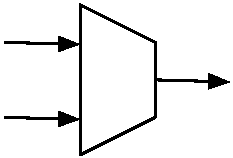
\includegraphics{figures/mux}

  \caption{A basic 2:1 multiplexor.}
  \label{fig:mux}
\end{figure}


\subsection{Counting}

Counting is a very basic operation in digital systems. On might count events.
However, more often counting is used to define a time interval. Counting the
clock cycles and triggering an action when the time interval has expired.

A simple approach is counting up to a value. However, in computer science,
and in digital design, counting starts at 0. Therefore, if we want to count till
10 we count from 0 to 9. The following code shows such a counter that counts
till 9 and wraps around to 0 when reaching 9.

If we want to count N, we start with 0 and count till N-1.

\todo{counter code}



This is straight forward. However, one might ask if this is the most efficient
implementation of counting. The comparison agains an end value, 10 in our
example, involves some combinational circuit in an ASIC. More efficient in an
ASIC (and as well in loops of programs) is counting down and exit when 0
is reached.

If we want to count N, we start with N-1 and count till 0.

\todo{down counting code}

With a comparison against 0 we need only a NOR gat to detect the 0 condition.
This optimization is valid for an ASIC, but not for an FPGA based on LUTs.
With comparison using LUTs there is no difference comparing against a '0' or
'1' bit. In that case use the better readable counting logic towards the end value.

However, there is still one more trick a clever hardware designer can pull off.
Counting up or down needed a comparison agains all counting bis, so far.
What about counting down \emph{one to many}? In that case the counter
becomes negative. Detecting a negative value is simply comparing the
most significant bit against 'a'.

If we want to count N, we start with N-2 and count till -1.

\todo{Show optimized down counting code.}


\todo{discuss >= and so on}

\section{Components}

\subsection{FIFO Buffer}

To decouple a write (sender) and a reader (receiver) some form
of buffering between the writer and the reader is inserted.
A common buffer is a first-in, first-out
(\href{https://en.wikipedia.org/wiki/FIFO_%28computing_and_electronics%29}{FIFO})
buffer. Figure~\ref{fig:fifo} shows a writer, the FIFO, and a reader.
Data is put into the FIFO by the writer on \code{din} with an active
\code{write} signal. Data is read from the the FIFO by the reader on
\code{dout} with an active \code{read} signal.

\begin{figure}
  \centering
  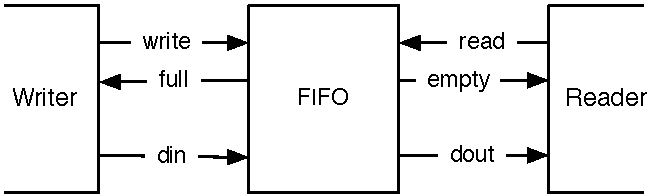
\includegraphics{figures/fifo}

  \caption{A writer, a FIFO buffer, and a reader.}
  \label{fig:fifo}
\end{figure}

A FIFO is initially empty, singled by the \code{empty} signal. Reading
from an empty FIFO is usually undefined. When data is written and never
read a FIFO will become \code{full}. Writing to a full FIFO is usually ignored
and the data lost. In other words, the signals \code{empty} and \code{full}
serve as handshake signals 

Several different implementations of a FIFO are possible: E.g., using on-chip
memory and read and write pointers or simply a chain of registers with a
tiny state machine. For small buffers (up to tens of elements) a FIFO organized
with individual registers connected into a chain of buffers is a simple and efficient
implementation.

We start by defining the IO signals for the writer and the reader. The size of
the data is configurable with \code{size}.

\begin{chisel}
class WriterIO(size: Int) extends Bundle {
  val din = UInt(INPUT, size)
  val write = Bool(INPUT)
  val full = Bool(OUTPUT)
}

class ReaderIO(size: Int) extends Bundle {
  val dout = UInt(OUTPUT, size)
  val read = Bool(INPUT)
  val empty = Bool(OUTPUT)
}
\end{chisel}


\section{Snippets}

\todo{A collection is Chisel snippets collected along some coding}


A memory with sequential registered read and write ports:
\begin{chisel}
  val mem = Mem(UInt(width = 8), 256, seqRead = true)
  val rdData = mem(Reg(next = rdAddr))
  when(wrEna) {
    mem(wrAddr) := wrData
  }
\end{chisel}

Initialize a \code{Vec} from a Scala array:
\begin{chisel}
  val program = new Array[Bits](3)
  program(0) = Bits(0x01, 8)
  program(1) = Bits(0x23, 8)
  program(2) = Bits(0x16, 8)
    
  val rom = Vec(program)
\end{chisel}

State machine:
\begin{chisel}
  val fetch :: execute :: load :: Nil = Enum(UInt(), 3)
  val stateReg = Reg(init = fetch)

  switch(stateReg) {
    is(fetch) {
      stateReg := execute
    }
    is(execute) {
      when(isLoad) {
        stateReg := load
      }.otherwise {
        stateReg := fetch
      }
    }
    is(load) {
      stateReg := fetch
    }
  }
\end{chisel}

\textbf{No default assignment possible when declaring a signal! Need an extra one.}

\subsection{SBT and Eclipse}

Use an IDE, such as Eclipse, but generate the project with \code{sbt}
from the library dependency description. E.g.,:

\todo{add Eclipse stuff here.}

\section{Conclusion}
\label{sec:conclusion}


\subsection*{Acknowledgment}

\todo{Sometimes we received some help. Sometimes external funding.}



\subsection*{Source Access}

All code examples are available in open source from:

\url{https://github.com/schoeberl/chisel-examples}

\bibliographystyle{plain}
% Please do not add any references to msbib.bib.
% They get lost when I 'generate' is again (see Makefile)
\bibliography{chisel}

\end{document}

\subsection{Course Abstract}

Chisel is a hardware construction language implemented as a domain specific language in Scala. Therefore, the full power of a modern programming language is available to describe hardware and, more important, hardware generators. Chisel has been developed at UC Berkeley and successfully used for several tape outs of RISC-V. Here at DTU we used Chisel in the T-CREST project and in teaching advanced computer architecture.

In this course I will give an overview of Chisel to describe circuits at the RTL, how to use the Chisel tester functionality to test and simulate digital circuits, present how to synthesize circuits for an FPGA, and present advanced functionality of Chisel for the description of circuit generators. Besides lecturing we will have lab sessions to describe small circuits and evaluate them in an FPGA.

The aim of the course is to get a basic understanding of a modern hardware description language and be able to describe simple circuits in Chisel. This course shall give a basis to explore more advanced concepts of circuit generators written in Chisel/Scala.

%\begin{figure}
%  \centering
%  \includegraphics{figures/broken-mux}
%
%  \caption{An inkscape figure. With arrows shooting over the destination coordinates!}
%  \label{fig:mux}
%\end{figure}